%%%%%%%%%%%%%%%%%%%%%%%%%%%%%%%%%%%%%%%%%%%%%%%%%%%%%%%%%%%%%%%%%%%%%%%%%%%%%%%%
%Objetivo: Propor um conjunto de recomendações de melhorias para as
% 		   as funcionalidade das FGRMs
%Autores: Vagner Clementino <vagnercs@dcc.ufmg.br>
%		  Rodolfo Resende <rodolfo@dcc.ufmg.br>
%Criação: dom fev 26 12:49:27 BRT 2017
%Modificação: sáb abr 15 12:54:15 -03 2017
%Revisão:
%%%%%%%%%%%%%%%%%%%%%%%%%%%%%%%%%%%%%%%%%%%%%%%%%%%%%%%%%%%%%%%%%%%%%%%%%%%%%%%%
\chapter{Sugestões de Melhorias para as FGRMs}
\label{ch:sug_melhoria}

\section{Introdução}
\label{sec:sug_melhoria_intro}

Os usuários das Ferramentas de Gerenciamento de Requisições de Mudança (FGRM),
se mostraram, em geral, satisfeitos com as funcionalidades oferecidas pela
ferramenta. Cerca de 90\% dos par\-ti\-ci\-pan\-tes do levantamento por
questionário descrito no Capítulo~\ref{ch:pesquisa-profissionais} fizeram uma
avaliação positiva e também afirmam que recomendariam a FGRM que utilizam para
um novo projeto.

Não obstante, naquele mesmo levantamento, ao questionarmos se o profissional
sentiria falta de alguma das funcionalidades que lhe foi apresentada, cerca de
85\% responderam positivamente, ou seja, afirmaram que as funções apresentadas
poderiam contribuir em sua rotina de trabalho. A partir desta última informação
podemos inferir que os desenvolvedores estão satisfeitos com a ferramenta
utilizada, contudo, \textit{não conhecem ou não têm acesso ao potencial de
	funções que este tipo software poderia oferecer}.

Diante do exposto, entendemos que podemos contribuir com o estado a\-tu\-al das
funcionalidades das FGRMs através da proposição de conjunto de melhorias.  As
sugestões foram compiladas utilizando os resultados obtidos nesta dissertação,
especialmente com base nos Capítulos~\ref{ch:mapeamento-sistematico}
e~\ref{ch:pesquisa-profissionais}, na Seção~\ref{sec:caracterizacao_ferramentas}
e nos estudos que propõem melhorias para as FGRM~\cite{zimmermann2009improving,
	bettenburg2008makes, singh2011bug}.  Estas recomendações podem ser
utilizadas por pesquisadores interessados em conduzir estudos sobre o avanço da
produtividade dos desenvolvedores mediante o uso das FGRMs. Além disso, os
responsáveis pela implementação deste tipo de software podem utilizar este
conjunto a fim de desenvolver futuras versões do sistema. Na mesma linha, os
profissionais envolvidos em manutenção de software podem criar extensões
(plugins) para as FGRM com base no que foi proposto de modo a utilizar as
melhorias propostas neste estudo em sua rotina de trabalho.

Este capítulo está organizado da seguinte forma: a
Seção~\ref{sec:sug_melhoria_melhorando_as_ferraementas} apresenta as sugestões
de melhorias do qual acreditamos poderia ser implantadas nas FGRMs, cada
sugestão foi seguida de uma breve discussão de como foi obtida e dos motivos de
sua implementação; na Seção~\ref{sec:sug_melhoria_avaliacao_das_melhorias}
realizamos a avaliação das sugestões que foram propostas, onde solicitamos a
opinião de profissionais que participam de projetos de código aberto que
desenvolvem FGRMs; na Seção~\ref{sec:sug_melhoria_discussao} discutimos os
resultados obtidos do processo de avaliação; na
Seção~\ref{sec:sug_melhoria_ameacas} apresentamos as ameaças à validade deste
capítulo; encerramos o capítulo com um resumo na
Seção~\ref{sec:sug_melhoria_resumo}.

\section{Sugestões de Melhorias para as FGRMs}
\label{sec:sug_melhoria_melhorando_as_ferraementas}

As sugestões propostas neste capítulo não estão vinculadas exclusivamente à
melhorias de funcionalidades existentes nas FGRMs. As recomendações podem
representar o desenvolvimento de um novo comportamento para este tipo de
ferramenta. Cabe-nos ressaltar que o conjunto proposto não é exaustivo e é
baseado nos resultados desta dissertação. Além disso, não houve compromisso com
as dificuldades operacionais relacionadas com a implementação das
funcionalidades.

Ao longo da elaboração das sugestões verificamos que não conseguiríamos
implementar todas elas. Além de decidirmos não desenvolver todas as sugestões
por entendemos que a análise desta complexidade está fora do escopo deste
estudo. Exceção foi a recomendação descrita na
Seção~\ref{sub:supote_a_qualidade_do_relato} foi implementada como extensão de
uma FGRM, conforme pode ser visto no Capítulo~\ref{ch:implemtacao_extensao}.  É
possível que algumas das su\-ges\-tões propostas já estejam implementadas de
maneira parcial ou integral em alguma FGRM\@. Contudo, não é possível validar
esta premissa por conta de volume de ferramentas disponíveis quando esta
dissertação foi escrita.Cada sugestão proposta foi estruturada como uma seção
deste capítulo onde apresentamos a \textit{justificativa, o benefício gerado, as
	limitações e alguns exemplos de utilização.}

\subsection{Suporte à Qualidade do Relato}
\label{sub:supote_a_qualidade_do_relato}

\sugestao{01}{As FGRMs devem fornecer um retorno da qualidade do relato
	realizado em uma RM.}

\paragraph{Justificativa:}
\label{par:justificativa_s01}

Conforme discutido na
Seção~\ref{subsec:man_visao_geral_papeis_na_manutencao_de_software} o
responsável por reportar uma RM pode ser tanto um usuário do sistema quando um
membro da equipe de desenvolvimento ou manutenção. Por esta razão, podemos
encontrar Reportadores com diferentes níveis de conhecimento sobre o sistema.
Este fato pode acarretar em níveis desiguais de qualidade do que será relatado,
o que causar atraso na análise da RM por falta da informação necessária a sua
resolução. Alguns estudos demonstram que, do ponto de vista dos desenvolvedores,
a falta de informação, tais como etapas para reproduzir a falha e registro de
pilha de ativação (stack track), dificultam mais o trabalho do que relato de
problemas (bugs) duplicados~\cite{bettenburg2008makes, bettenburg2007quality}.
Nesta linha, alguns trabalhos se propõem a minimizar este problema através da
análise da qualidade do que é relatado em uma RM\@. A premissa é que o
responsável por criar uma RM deva ter ciência das informações para a sua
solução\footnote{A descrição do que entendemos por solução de uma RM pode ser
	encontrado no Capítulo~\ref{ch:visao-geral-manutencao}}.

\paragraph{Benefício Gerado:}
\label{par:beneficio_s01}

Com este tipo de funcionalidade uma FGRM poderia reduzir o tempo de análise de
determinada RM pelo fato que o responsável por cria-la estaria ciente das
informações necessárias à sua resolução. Neste caso, o benefício direto seria ao
desenvolvedor que teria a sua disposição um relato mais completo. Não obstante,
um trabalho adicional seria dado ao reportador que algumas situações devem rever
as informações incluídas na RM\@.

\paragraph{Limitações:}
\label{par:limitacoes_s01}

Alguns estudos sobre melhoria do qualidade do relato da RM focam
prioritariamente naquelas que se referem a defeitos do software. Conforme
discutimos na Seção~\ref{sec:requisicao_de_mudanca}, além do relato de um
problema uma RM também incluí pedidos de melhoria. Dada estas duas dimensões,
nem sempre é possível avaliar a qualidade do relato por conta de suas diferentes
e necessidades.

\paragraph{Exemplo de Utilização:}
\label{par:exemplo_s01}

Após o usuário relatar um problema em determinada FGRM, a ferramenta de imediato
avalia a RM gerada e apresenta ao responsável pelo relato algumas dicas de como
a informação fornecida poderia ser melhorada, como por exemplo através da
inclusão de um arquivo com o histórico de execução do software (log).

\subsection{Busca por Código Fonte}
\label{sub:busca_por_código_fonte}

\sugestao{02}{As FGRMs devem possibilitar a busca por código fonte contido em
	seu relato, comentários ou anexos.}

\paragraph{Justificativa:}
\label{par:justificativa_s02}

As RMs permitem a inserção de código fonte em diversas etapas do seu ciclo de
vida. O código pode ser incluído durante a sua criação, nas discussões
realizadas para a sua resolução ou mesmo quando ela é concluída, onde recebe o
nome de \textit{patch.} Esta informação é bastante relevante para o projeto do
qual a RM faz parte, contudo, as FGRMs não permitem a sua recuperação.

\paragraph{Benefício Gerado:}
\label{par:beneficios_s02}

Caso o desenvolvedor ou analista de qualidade possa facilmente acessar o código
fonte utilizado para exemplificar ou corrigir determinada RM, eles podem
utilizar esta informação para solucionar outras RMs que possam ter relação com
a primeira. Este tipo de funcionalidade pode ser vantajosa em comparação a uma
busca estruturada, presente em grande parte deste tipo de software, por permitir
a busca de elementos específicos da linguagem que é utilizada pelo software que
a FGRM suporta, como por exemplo classes, funções, constantes e outros.

\paragraph{Exemplo de Utilização:}
\label{par:exemplo_s02}

Um desenvolvedor ao verificar que a RM que ele esteja tratando é similar a outra
anteriormente relatada, ele pode buscar pelo código fonte que foi utilizado para
resolver a primeira.

\subsection{Diferenciação do Reportador}
\label{sub:diferenciacao_do_reportdor}

\sugestao{03}{As FGRMs devem diferenciar as RMs criadas por reportadores que
	historicamente relatam com qualidade e relevância.}

\paragraph{Justificativa:}
\label{par:justificativa_s03}

Caso seja possível identificar que um \textit{Reportador} tem por hábito relatar
RMs que sejam relevantes ao projeto de software, tais requisições deveriam
receber algum tipo de etiqueta de modo a diferenciá-las dentro da FGRM\@.
Segundo o nosso entendimento uma RM pode ser classificada como relevante se
descreve um problema que afeta um grande número de usuários do sistema ou
representa uma falha de segurança do software. Além disso deve ser redigida de
forma clara e fornecer as informações necessárias para sua solução. O grau de
relevância de determinada RM pode variar em diferentes projetos e pode depender
de critérios subjetivos de quem analisa.

\paragraph{Benefício Gerado:}
\label{par:papéis_afetados_s03}

O papel de agendador é responsável por definir o desenvolvedor mais apto
para determinada RM utilizando diversos critérios como por exemplo a prioridade
do que foi relatado. Esta atividade pode receber uma ajuda caso uma RM possua
alguma diferenciação que demostre que foi criada por um reportador que
frequentemente o faz com relevância. Essas RMs podem receber uma maior atenção
de modo a ser priorizada.

\paragraph{Exemplo de Utilização:}
\label{par:exemplo_de_utilização_s03}

Um agendador ao verificar uma RM que é capaz de ser diferenciada tomando por
base que a relatou poderia priorar aquela RM ou mesmo realizar pesquisas prévias
com este tipo de classificador. Com objetivo de diferenciar as RMs deste perfil
de reportadores apresentamos a \textit{Sugestão 03}.

\subsection{Histórico das Últimas RMs}
\label{sub:histórico_das_ùltimas_rm_s}

\sugestao{04}{As FGRMs devem permitir acesso facilitado para as $n$ últimas RMs
	que foram analisadas por um desenvolvedor.}

\paragraph{Justificativa:}
\label{par:justificativa_s04}

No ciclo de vida de uma RM, conforme discutido na
Subseção~\ref{subsec:man_visao_geral_papeis_na_manutencao_de_software}, após a
verificação de que a RM foi incorporada com sucesso ao software, ela é movida
para o estado \textit{Fechado (Closed)} e deixa de estar atribuída a determinado
desenvolvedor ou analista de qualidade. Caso um desenvolvedor queira acessá-la
novamente deverá utilizar o identificador da RM a fim de recuperá-la na FGRM\@.
Este histórico de trabalho do desenvolvedor pode ser útil na resolução de
eventuais RM que surjam posteriormente no projeto. No levantamento mediante
questionário, apresentado no Capítulo~\ref{ch:pesquisa-profissionais}, alguns
participantes relataram o desejo de uma funcionalidade  que gerencie este
histórico conforme apresentado a seguir.

\begin{itemize}
	\item Conforme relato dos participantes eles gostariam:
	\begin{itemize}
		\item \textit{``The ability to clearly visualize how many tickets are at
				the to do, in progress, to validate or done steps.''}.
		\item \textit{``History tracking, commenting, attachments, priority
				setting, task assignment, tie in with deployment systems.''}
	\end{itemize}
\end{itemize}

\paragraph{Benefício Gerado:}
\label{par:papéis_afetados_s04}

Com o acesso às últimas RMs analisadas o desenvolver tem uma noção do trabalho
desenvolvido e a um conjunto de informações que podem ser utilizadas para
resolver as RMs que estão sob sua responsabilidade.

\paragraph{Exemplo de Utilização:}
\label{par:exemplo_de_utilização_s04}

Ao acessar a FGRM o desenvolvedor tem acesso as últimas $n$ RMs que ele
analisou. Para facilitar a visualização este numero pode ser fixado em valores
tais como $n = {5, 10, 30}$.

\subsection{Suporte à Integração Contínua}
\label{sub:suporte_integracao_continua}

\sugestao{05}{Integração Contínua}

\paragraph{Justificativa:}
\label{par:justificativa_s05}

Dentro da disciplina de Gerência de Configuração, a \textit{Integração Contínua}
(IC) é a prática de construir (build) e implantar (deploy) imediatamente após um
desenvolvedor consolidar (commit) o código fonte para o
repositório~\cite{aiello2010configuration}. A IC tornou-se dentro das práticas
propostas pelos agilistas e vêm ganhando popularidade em ambientes de
desenvolvimento mais tradicionais. Um possível gatilho para o processo de IC
poderia ser a solução de uma RM, que em determinados contexto é feito pela
alteração da situação da RM para \textit{Fechada} \@-\@ uma discussão sobre o
ciclo de vida das RMs pode ser encontrada na
Seção~\ref{sub:sub:fluxo_de_trabalho_requisicao_mudanca}. Desta forma, seria
possível mapear uma versão do sistema com o conjunto de RMs solucionadas até a
sua geração. Este tipo de integração foi descrita como uma possível
funcionalidade ausente nas FGRMs por alguns participantes do levantamento por
questionário descrito no Capítulo~\ref{ch:pesquisa-profissionais}.

\paragraph{Benefício Gerado:}
\label{par:papéis_afetados_s05}

A integração de uma FGRM com outras ferramentas de IC traria ao processo de
manutenção os benefícios desta prática, tais como redução de riscos e facilidade
de encontrar e remover falhas~\cite{fowler2006continuous}.  Além disso, segundo
o nosso entendimento, o fato de vincular a solução de uma RM com determinada
versão de um sistema, pode minimizar problemas levantados no Mapeamento
Sistemático descrito no Capítulo~\ref{ch:mapeamento-sistematico} tais como
Localização do Problema (Seção~\ref{ssub:melhorias_dim_ferramenta}) e Estimativa
de Esforço da RM (Seção~\ref{ssub:melhorias_dim_processo}). Em ambos os casos é
possível aproveitar da facilidade que a IC fornecer em a localização de uma
falha que, por exemplo, pode ter sido causada pela solução de uma RM\@.

\paragraph{Limitações:}
\label{par:limitacoes_s05}

Algumas vezes a mudança de situação de uma RM para \textit{Fechada} pode não
representar a sua solução.


\paragraph{Exemplo de Utilização:}
\label{par:exemplo_de_utilização_s05}

The results of the build are posted on a dashboard, including the most recent
changes responsible for any system outages, including a failed build

\subsection{Suporte à Linguagem de Marcação}
\label{sub:suporte_linguagem_marcacao}

\sugestao{06}{Suporte a linguagem de marcação}

\paragraph{Justificativa:}
\label{par:justificativa_s06}

\paragraph{Benefício Gerado:}
\label{par:papéis_afetados_s06}

\paragraph{Limitações:}
\label{par:limitacoes_s06}

\paragraph{Exemplo de Utilização:}
\label{par:exemplo_de_utilização_s06}

\subsection{Priorização automática de RMs}
\label{sub:priorizacao_automatica_rms}

\sugestao{07}{Priorização automática de RMs urgente e não esperadas}

\paragraph{Justificativa:}
\label{par:justificativa_s07}

\paragraph{Benefício Gerado:}
\label{par:papéis_afetados_s07}

\paragraph{Limitações:}
\label{par:limitacoes_s07}

\paragraph{Exemplo de Utilização:}
\label{par:exemplo_de_utilização_s07}

\subsection{Suporte à Reuniões Diárias (Daily)}
\label{sub:suporte_reunicao_diarias}

\sugestao{08}{Ajuda do desenvolvedor em sua reunião diária (daily)}

\paragraph{Justificativa:}
\label{par:justificativa_s08}

\paragraph{Benefício Gerado:}
\label{par:papéis_afetados_s08}

\paragraph{Limitações:}
\label{par:limitacoes_s08}

\paragraph{Exemplo de Utilização:}
\label{par:exemplo_de_utilização_s08}

\subsection{Suporte à tarefas compartilhadas}
\label{sub:suporte_tarefas_compartilhadas}

\sugestao{09}{Suporte a tarefas compartilhadas foram as mais frequentes}

\paragraph{Justificativa:}
\label{par:justificativa_s09}

\paragraph{Benefício Gerado:}
\label{par:papéis_afetados_s09}

\paragraph{Limitações:}
\label{par:limitacoes_s09}

\paragraph{Exemplo de Utilização:}
\label{par:exemplo_de_utilização_s09}



\section{Avaliação das Melhorias Propostas}
\label{sec:sug_melhoria_avaliacao_das_melhorias}

Este Capítulo se propôs apresentar um conjunto de sugestões que foram
construídas tomando como base a literatura da área e os resultados e
contribuições desta dissertação. Com o objetivo de avaliar a relevância e o grau
de facilidade de implementação das recomendações propostas, conduzimos um
levantamento mediante questionário com profissionais que contribuem em projeto
de código aberto hospedados no Github. A metodologia utilizada na condução do
levantamento é descrita na próxima subseção.

\subsection{Metodologia Levantamento com Questionário}
\label{sub:sug_melhoria_metodologia_levantamento}

Para realizarmos a coleta dos dados foi utilizado um levantamento (survey)
através de um questionário eletrônico. O processo de seleção dos participantes,
o desenho do questionário e como foi realização a sua aplicação estão descritos
na próximas subseções.

\subsubsection{Seleção dos Participantes}
\label{ssub:sug_melhoria_selecao_participantes}

Ficou definido que o público-alvo deste questionário seria profissionais que
estejam ligados ao processo de desenvolvimento e manutenção de FGRMs. Este
perfil foi selecionado porque permite avaliar a relevância das sugestões
propostas ao mesmo tempo que possibilita verificar a viabilidade de
implementação do que foi recomendado em funcionalidades para as FGRMs. Por esta
razão, selecionamos profissionais que atuam como \textit{contribuidores} em três
projetos de código aberto hospedados no Github.

Com cerca de 38 milhões de
repositórios\footnote{\url{https://github.com/features}. Acesso em junho/2016.},
Github é atualmente o maior repositório de código na Internet. Sua popularidade
e a disponibilidade de metadados, acessíveis através de uma API, tem tornado
Github bastante atrativo para a realização de pesquisas na área de Engenharia de
Software.

Para escolha dos projetos foi definido inicialmente um conjunto de critérios
baseados em boas práticas recomendadas na literatura~\cite{Bird2009}. Em
síntese, um projeto para ser escolhido deve atender simultaneamente
aos seguintes requisitos:

\begin{itemize}
	\item Os projetos devem representar o desenvolvimento de uma FGRM\@.
	\item Os projetos devem ter no mínimo seis meses de desenvolvimento, para
		evitar projetos que não tenham passado por um tempo de manutenção
		relevante.
	\item Os projetos devem  ter  no  mínimo  200  revisões (commits)  pelos
		mesmos motivos  da restrição anterior.
	\item Os projetos escolhidos não devem ser ramificações (\textsl{branches}) um
		do outro projeto, para evitar dados duplicados.
	\item Os projetos obtidos devem ser os 10 mais populares que atendem aos
		demais critérios, utilizando como métrica o campo \texttt{most stars}
\end{itemize}

Após aplicação dos critérios descritos obtivemos os projetos descritos na
Tabela~\ref{tab:projetos_utilizados_para_avaliacao}. Conforme pode ser observado
os projetos selecionados referem-se a ferramentas bem estabelecidas e largamente
utilizadas por organizações e projetos de código aberto.

\begin{table}[htpb]
\centering
\resizebox{\textwidth}{!}{%
\begin{tabular}{@{}cccccc@{}}
\toprule
\textbf{Projeto} & \textbf{Revisões} & \textbf{Ramificações} &
\textbf{Lançamentos} & \textbf{Contribuidores} & \textbf{Contrib.\ com E-mail} \\
\midrule
bugzilla & 9784 & 30 & 460 & 100 & 30 \\
mantisbt & 10181 & 8 & 65 & 80 & 32 \\
redmine & 13115 & 27 & 131 & 6 & 2 \\ \bottomrule
\end{tabular}%
}
\caption{Projetos utilizados no levantamento com profissionais. Os dados
	apresentados tem como referência 07/03/2017.}
\label{tab:projetos_utilizados_para_avaliacao}
\end{table}

Com base nos projetos selecionados ficou definido que a amostra a ser utilizada
no levantamento seria os respectivos contribuidores. Um contribuidor é alguém
que participa efetivamente do desenvolvimento de um projeto, tendo o privilégio
de acesso para alterar o código fonte. O contato com os contribuidores foi
realizado por correio eletrônico, todavia, conforme pode ser verificado na
coluna \textit{Contrib.\ com E-mail} nem todos permitem acesso público ao seu
endereço. A Figura~\ref{fig:redmine_contribuidores} exibe uma página do projeto
com seus respectivos colaboradores.

\begin{figure}[htpb]
	\centering
	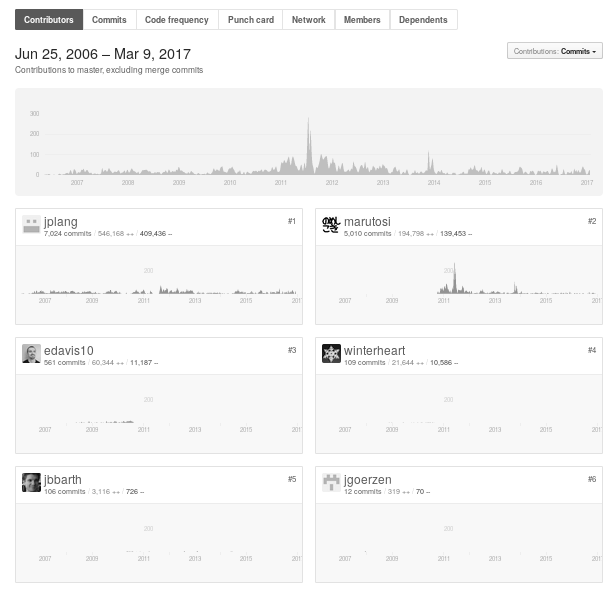
\includegraphics[width=0.8\linewidth]{./chapter-sugestoes-melhorias-fgrm/img/redmine_contribuidores.png}
	\caption{Lista de contribuidores do projeto Redmine}
\label{fig:redmine_contribuidores}
\end{figure}

\subsubsection{Desenho do Questionário}
\label{ssub:sug_melhoria_desenho_questionario}

A fim de coletar a opinião dos participantes foi utilizado um questionário
eletrônico produzido através da ferramenta \textit{Survey
	Gizmo}\footnote{\url{https://surveygizmo.com}}. O questionário foi desenhado
com a premissa de ser respondido em um prazo curto, de preferência entre 5 e 10
minutos. Neste sentido as perguntas foram organizadas em dois grupos principais.
As questões do primeiro grupo têm por objetivo coletar a opinião dos
profissionais sobre a relevância da recomendação proposta e o grau de
dificuldade de implementá-la. As perguntas foram estruturadas como uma escala
Likert em que o respondente deveria fornecer o seu nível de concordância para as
declarações que lhe são apresentadas. No segundo grupo as perguntas visam
estamos interessados na formação de base (background) dos profissionais. Optamos
por definir cada uma das questões como não obrigatórios por entendermos que a
impossibilidade ou o não interesse em responder uma determinada pergunta impeça
ao participante de enviar os dados de outras que foram respondidas. A
Figura~\ref{} exibe uma parte do formulário utilizado neste estudo.

\todobegin{Incluir figura com o formulário}

\subsubsection{Processo de Aplicação}
\label{ssub:processo_de_aplicação}

O questionário foi encaminhado à amostra de interesse através de correio
eletrônico. O endereço foi coletado diretamente do projeto hospedado no Github.
Foi desenvolvido um \textit{script} na linguagem Python que permitia coletar o
endereço de e-mail e automatizar o processo de envio. As mensagem foram
personalizadas de modo a identificar o nome do usuário e o projeto do Github
com base no template exibido a seguir.

\todobegin{Incluir o quadro com o template de envio das mensagens.}

O processo de envio consistia ainda de uma segunda mensagem de ``lembrete'' após
dois dias. Esta estratégia foi adotada com base em estudos que discutem
resultados em que o reenvio pode ser um dos fatores que aumentem a taxa de
participação em levantamentos por questionários realizados através da
web~\cite{fan2010factors}.

\section{Discussão}
\label{sec:sug_melhoria_discussao}

\section{Ameaças à Validade}
\label{sec:sug_melhoria_ameacas}

Foco em gente[contribuidores] que trabalha com ferramentas que são
``mainstream'' e portanto têm o viés de visão mais ``tradicional'' (ou outras
caracterizações que podem ser defendidas)

\section{Resumo do Capítulo}
\label{sec:sug_melhoria_resumo}
